\documentclass[12pt,letterpaper, onecolumn]{exam}
\usepackage{amsmath}
\usepackage{amssymb}
\usepackage{graphicx}
\usepackage{caption}
\graphicspath{ {./images/PS2} }
\usepackage[lmargin=71pt, tmargin=1.2in]{geometry}
\lhead{Mustafa Rashid\\}
\rhead{Problem Set 2\\}
\chead{\hline} 
\thispagestyle{empty} 
\newcommand*{\setdef}[1]{\left\{#1 \right\}} 

\begin{document}
	
	\begingroup  
	\centering
	\LARGE Multi-variable Calculus\\
	\LARGE Problem Set 2\\[0.5em]
	\large \today\\[0.5em]
	\large Mustafa Rashid\par
	\large Fall 2024\par
	\endgroup
	\rule{\textwidth}{0.4pt}
	\pointsdroppedatright
	\printanswers
	\renewcommand{\solutiontitle}{\noindent\textbf{Ans:}\enspace}  
	
	
	\begin{questions}
		
		\question Sketch (by hand) a contour diagram for the function $f(x,y) = -x^2-y^2+1$ with labeled contours $c = 0, -1, -2, -3, -4$. Draw at least four contour curves. Then write a sentence that describes the shapes of the contours and how they are spaced relative to each other.
		\begin{solution}
			\begin{center}
			\begin{tabular}{ c c  }
				$c$& $f(x,y)$\\
			0 & $x^2+y^2=1$ \\
			-1 & $x^2+y^2=0$ \\
			-2 & $x^2+y^2=3$ \\
			-3 & $x^2+y^2=4$ \\
			-4 & $x^2+y^2=5$ \\
			\end{tabular}
			\end{center}
			Concentric circles at (0,0) that get closer together as c decreases from 0 to -4.\\
			\makebox[0pt][l]{
				\begin{minipage}{\textwidth}
					\centering
					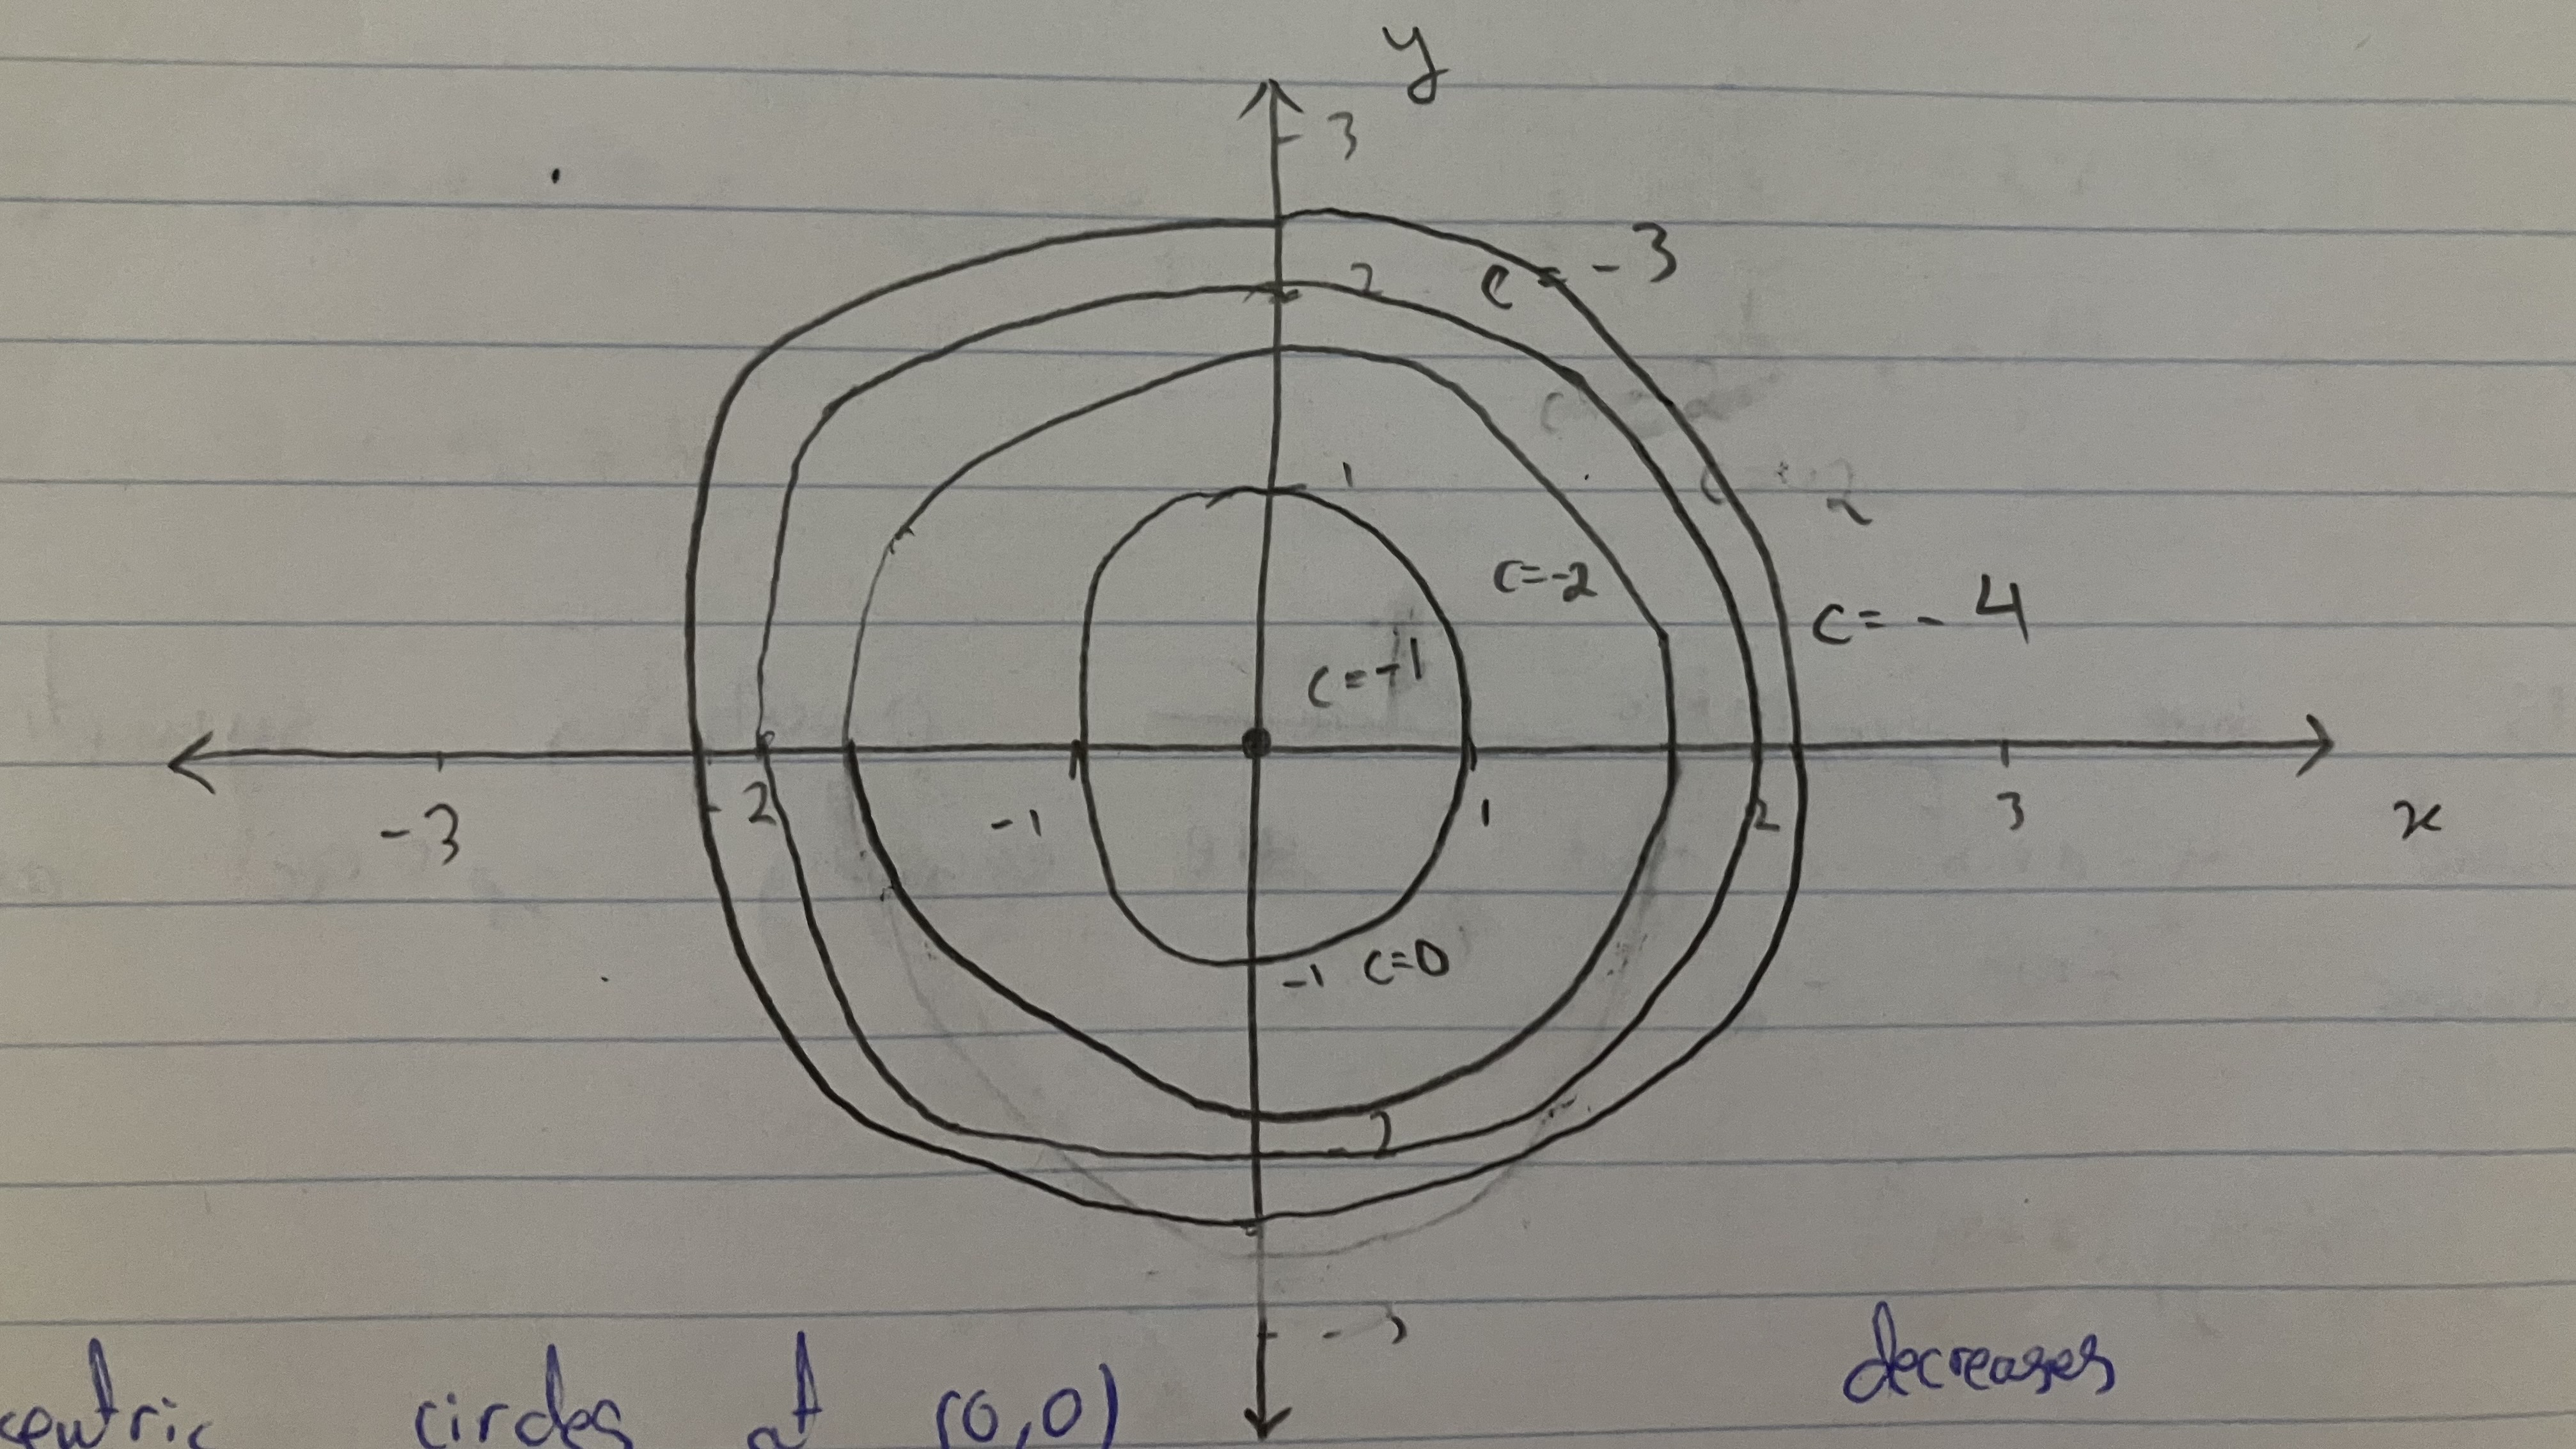
\includegraphics[width=.4\textwidth]{question1}
					\captionof{figure}{}
				\end{minipage}
			}
			\end{solution}
					\pagebreak
		\question Repeat the instructions of Question (1) for the function $f(x,y) = y-x^2$ and the contours $c = -2, -1, 0, 1, 2$.
		\begin{solution}
				\begin{center}
				\begin{tabular}{ c c  }
					$c$& $f(x,y)$\\
					-2 & $y=x^2-2$ \\
					-1 & $y=x^2-1$ \\
					0 & $y=x^2$ \\
					1 & $y=x^2+1$ \\
					2 & $y=x^2+2$ \\
				\end{tabular}
			\end{center}
			Contours are parabolas symmetric around $y$-axis that are equally spaced as $c$ changes from $-2$ to $2$\\
			\makebox[0pt][l]{
				\begin{minipage}{\textwidth}
					\centering
					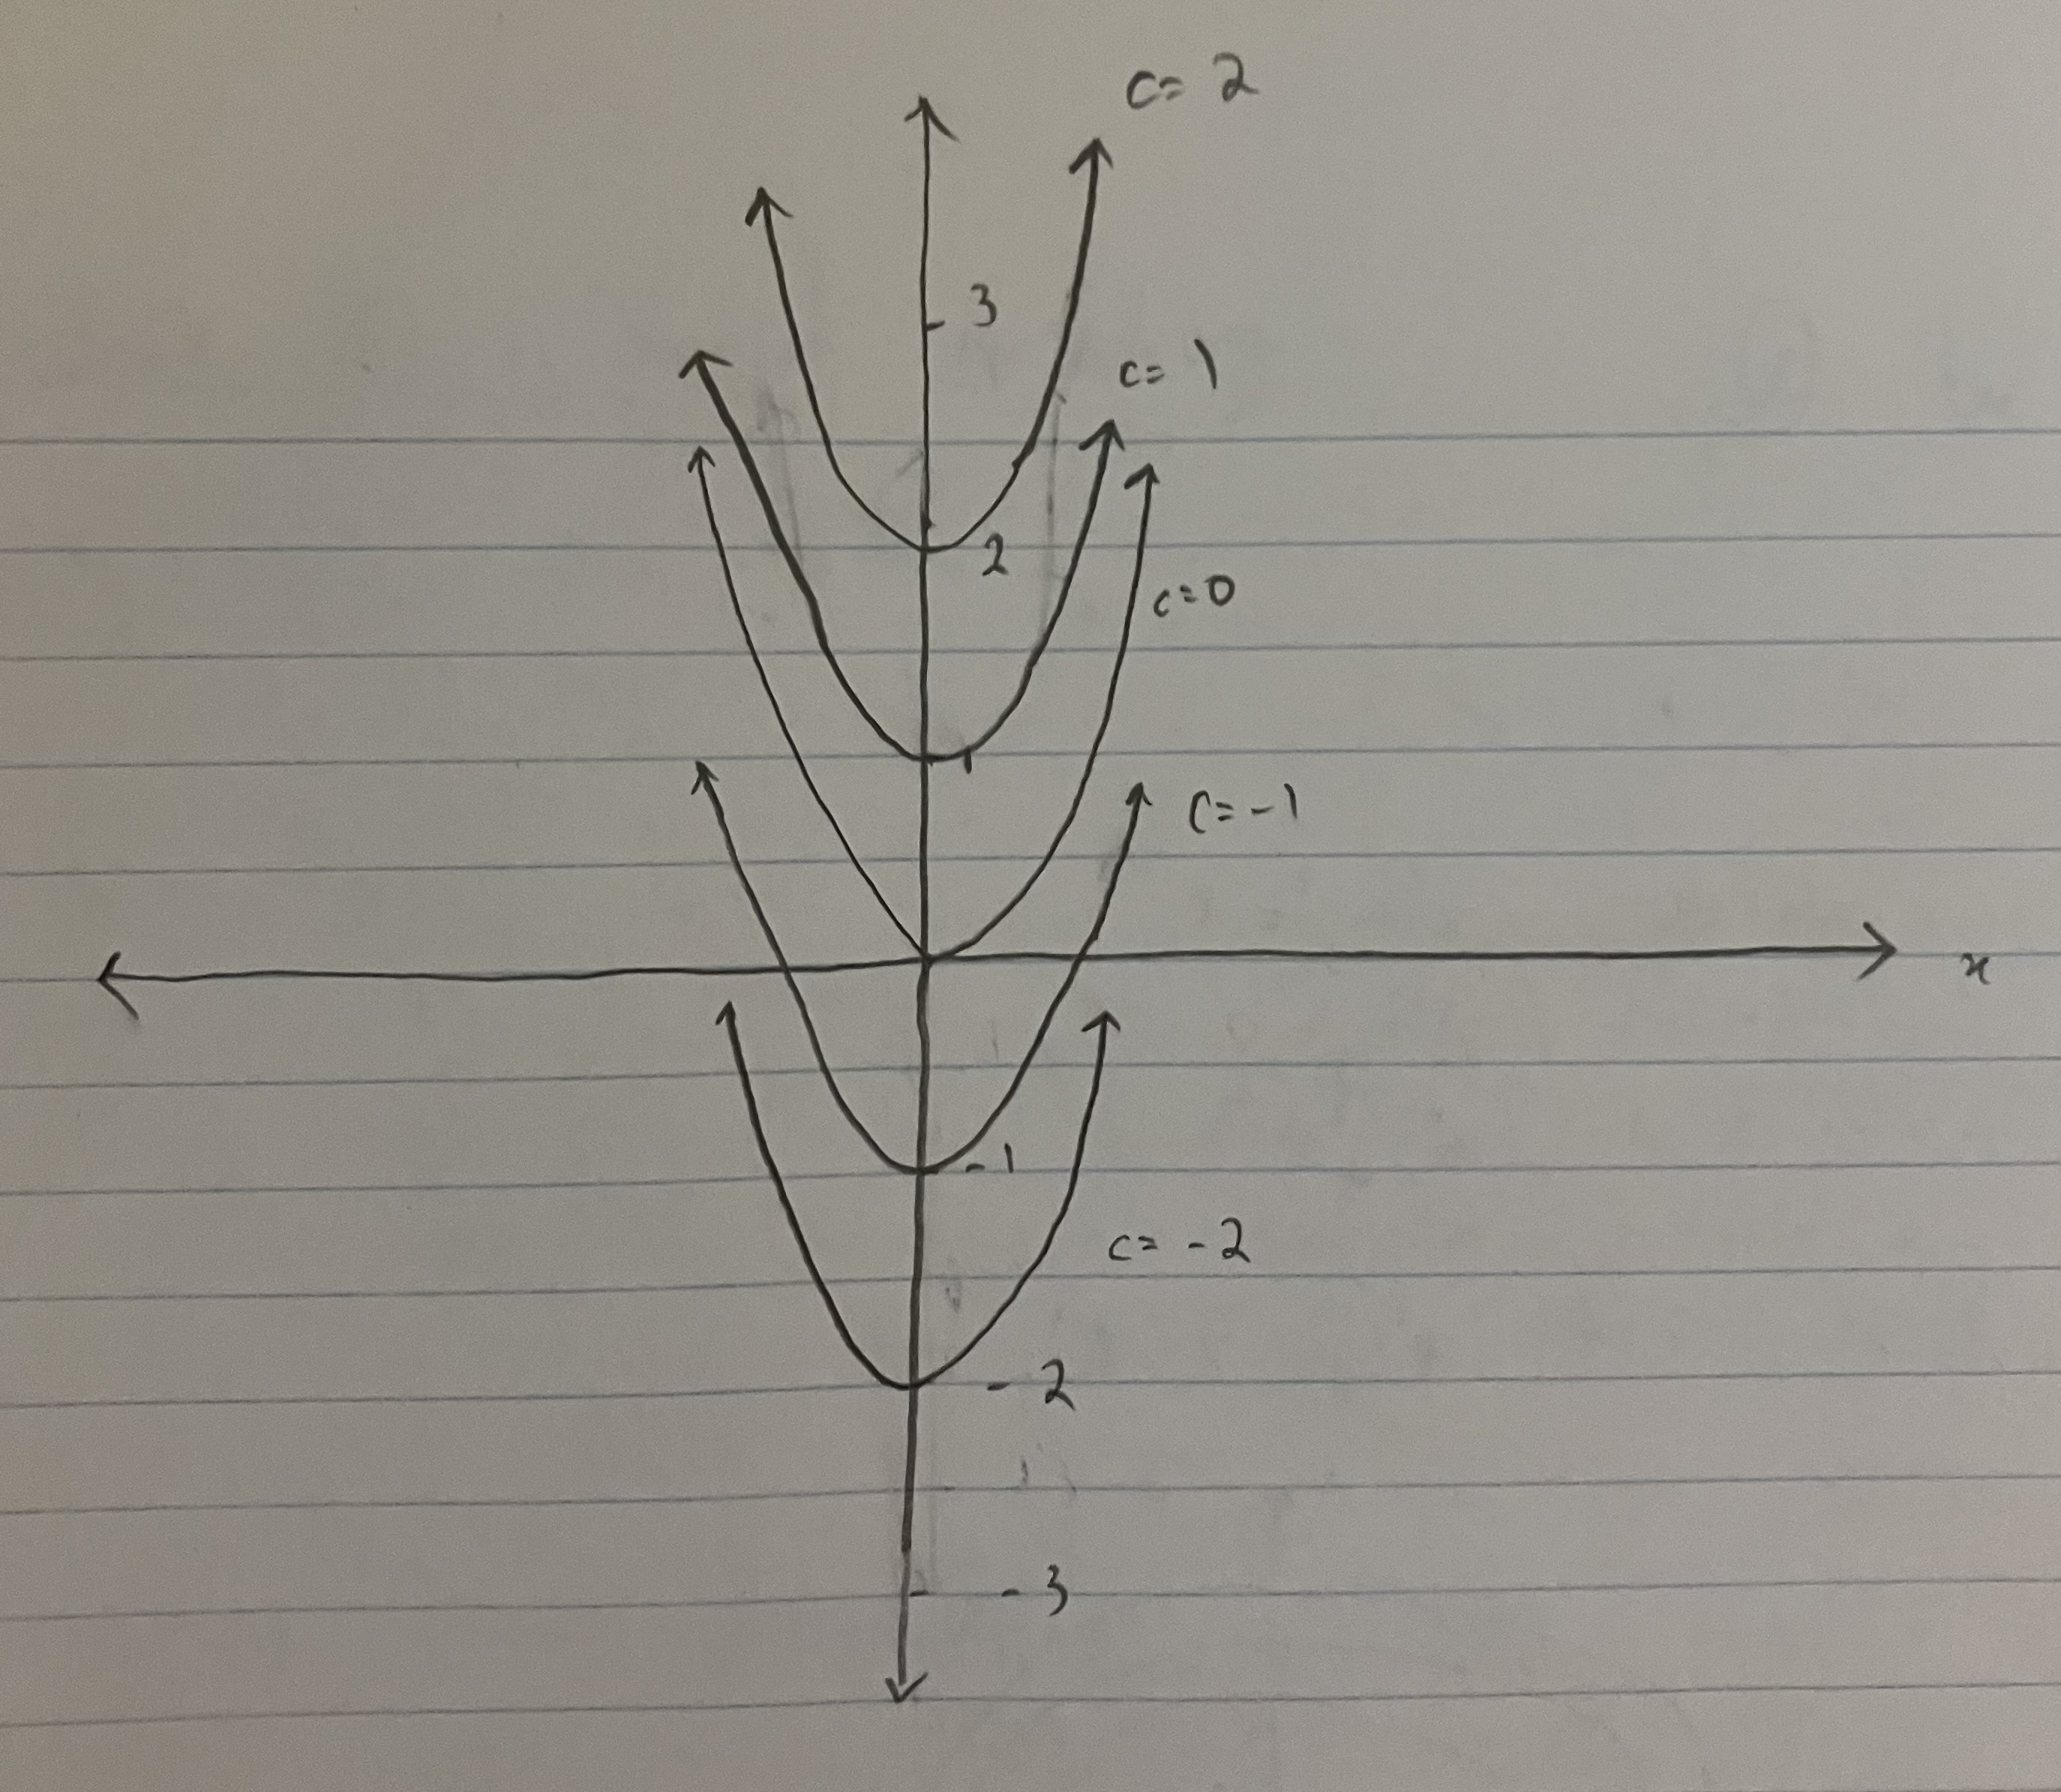
\includegraphics[width=.4\textwidth]{question2}
					\captionof{figure}{}
				\end{minipage}
			}
		\end{solution}
		
		\question Let $f(x,y)= x^2-y^2 = (x-y)(x+y)$. Use the factored form to sketch the contour given by $f(x,y)=0$ and to find the regions in the $xy$-plane where $f(x,y)>0$ and the regions where $f(x,y)<0$. Explain how this sketch shows that the graph of $f(x,y)$ is saddle-shaped at the origin.
		\begin{solution}
			From the factored form we can see that for $f(x,y)$ to be more than 0 both $(x-y)$ and $(x+y)$ need to be more than 0 or both need to be less than 0\\
			$f(x,y)$ is positive when $(x-y)>0$ and $(x+y)>0$ or  $(x-y)<0$ and $(x+y)<0$\\
			On the other side for $f(x,y)$ to be less than 0 we need $(x-y)<0$ and $(x+y)>0$ or  $(x-y)>0$ and $(x+y)<0$\\
			Since the contours are the lines $y=x$ and $y=-x$ we see that $f(x,y)$ is negative when $y>x$ and $y>-x$ or when $y<x$ and $y<-x$\\
			We also see that $f(x,y)$ is positive when $x>y$ and $x>-y$ or when $x<y$ and $x<-y$\\
			The fact that $f(x,y)$ is saddle shaped at the origin can be seen when looking at how the contour values change if we move in any of the 4 sections on the origin. Above and below the point $(0,0)$ the contours are negative meaning we are at shallower points but to the right and left of the point $(0,0)$ we have positive contours meaning that we are at higher points.\\
			\makebox[0pt][l]{
				\begin{minipage}{\textwidth}
					\centering
					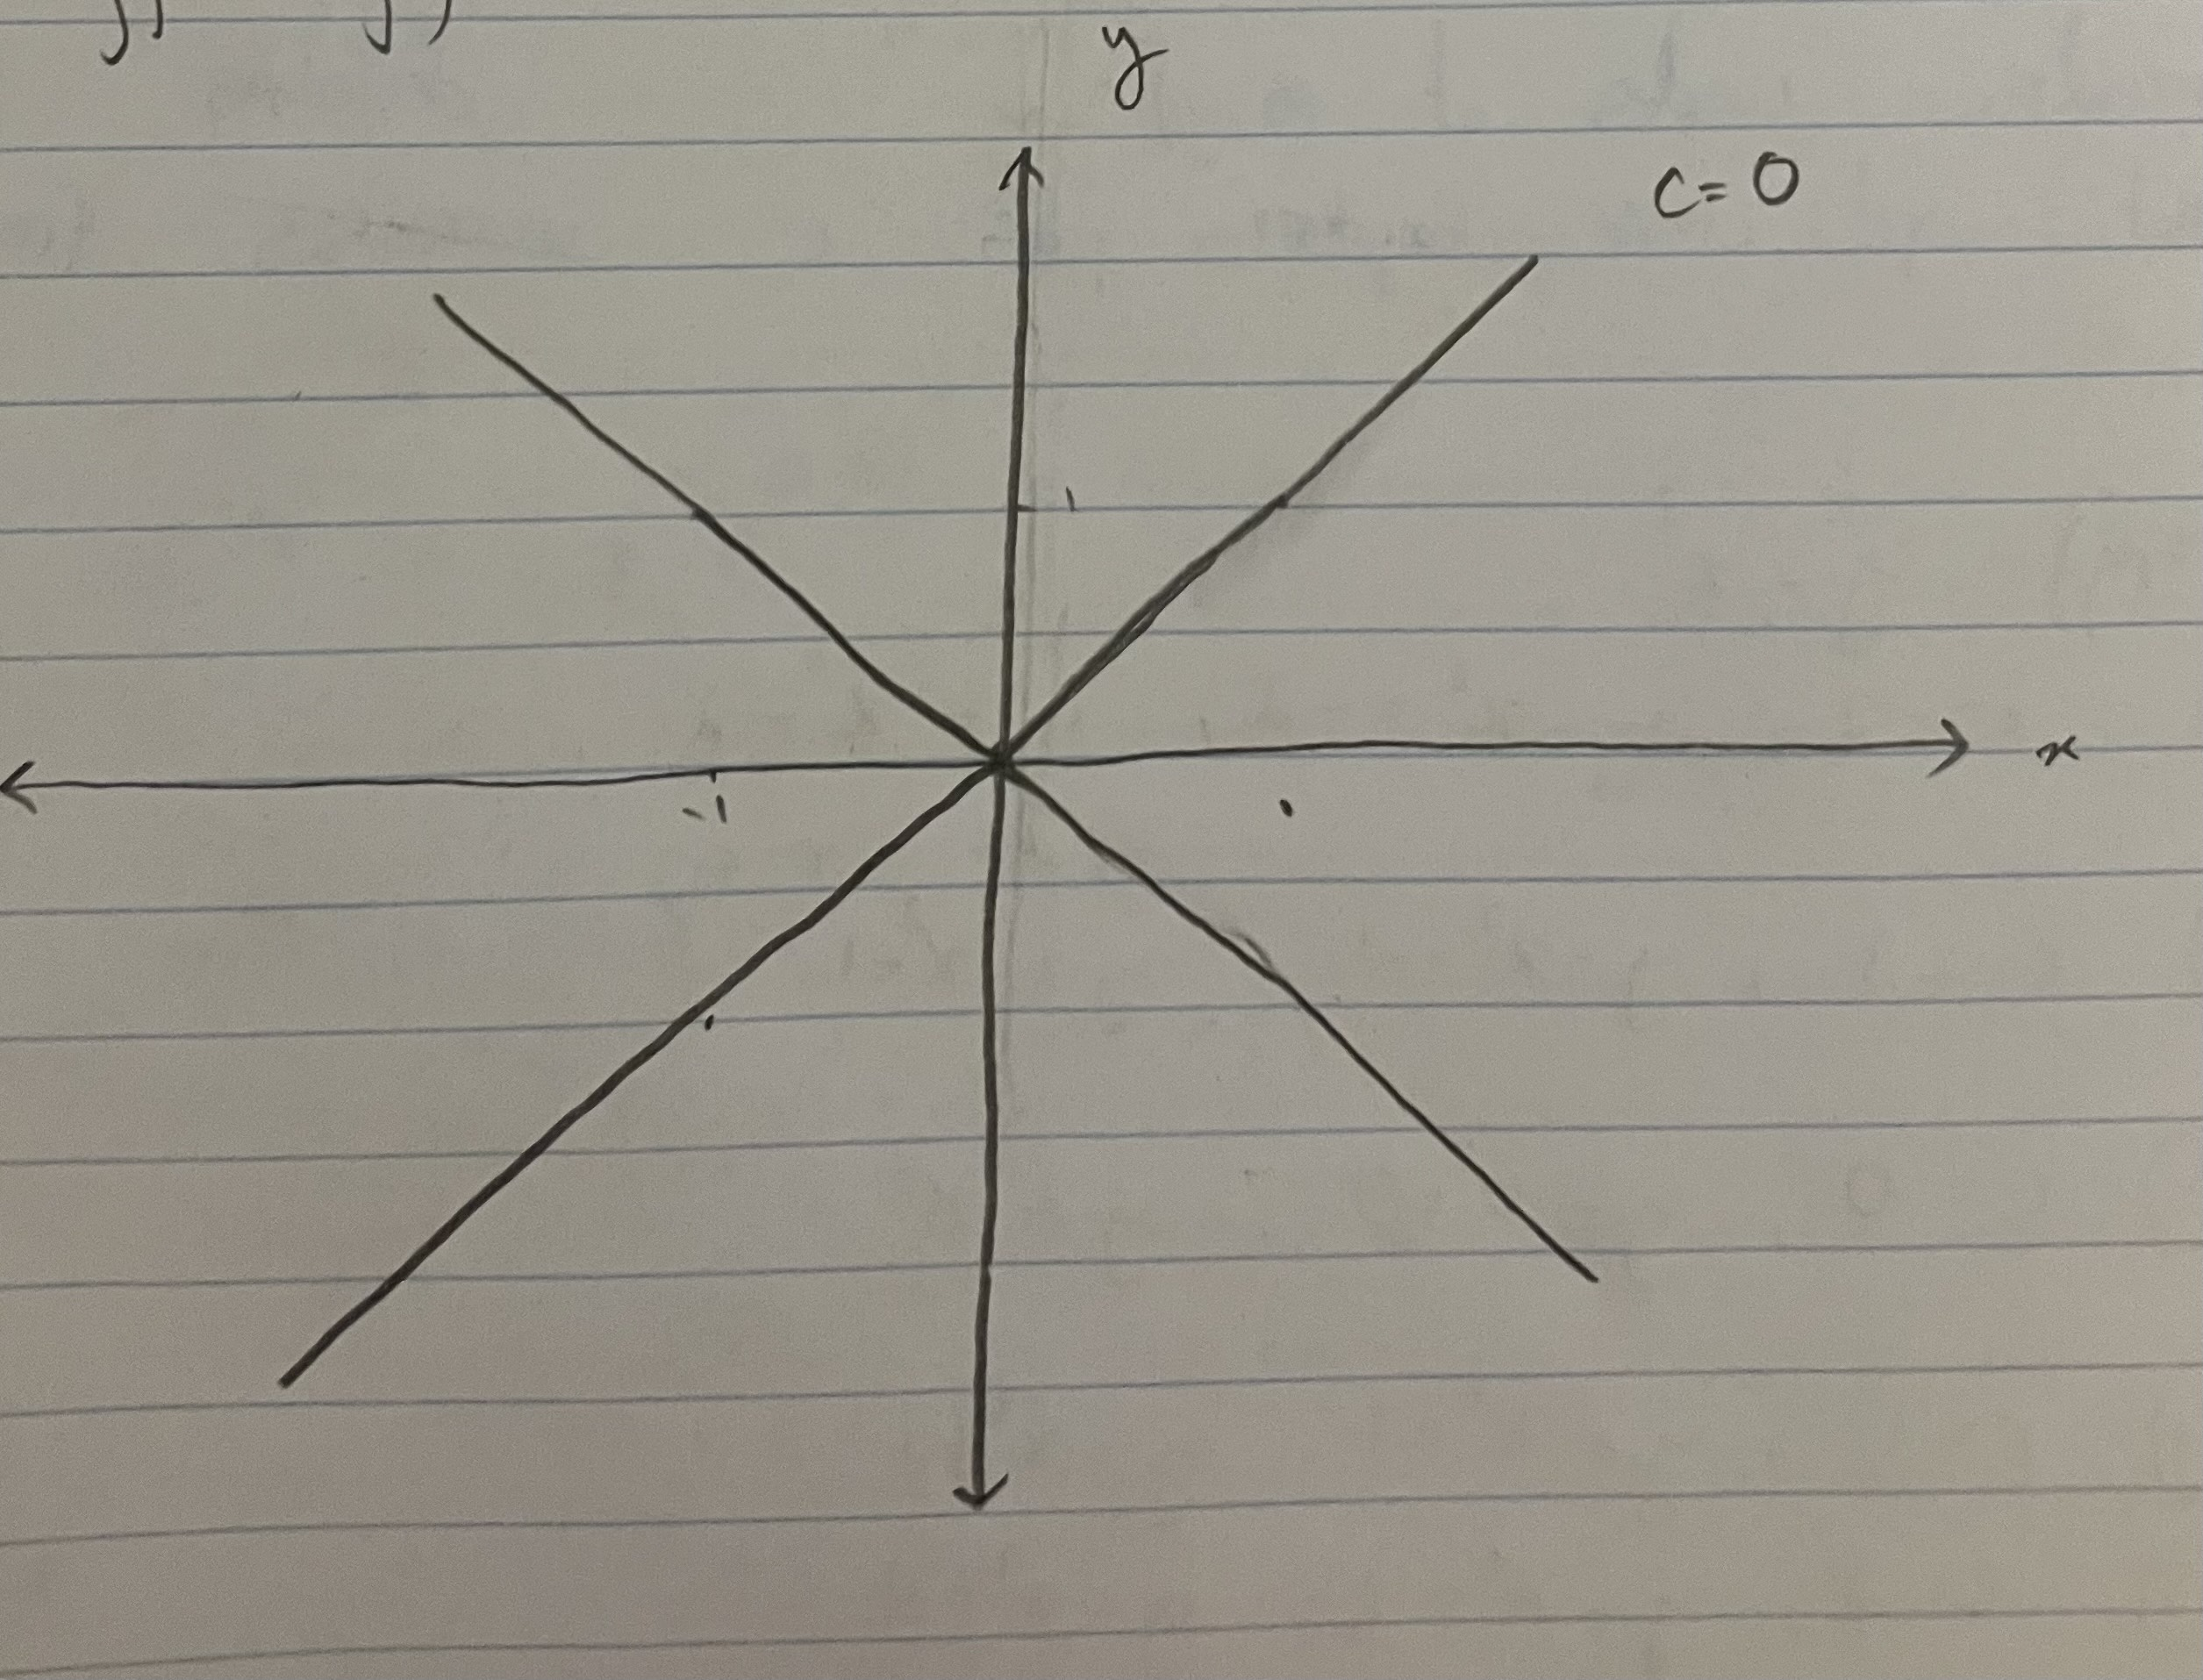
\includegraphics[width=.4\textwidth]{question3}
					\captionof{figure}{}
				\end{minipage}
			}
		\end{solution}
		
		\question The figure on the next page shows the contour plot of a linear function $f(x,y)$. Find the formula for the linear function and express it in \textit{Slope-Intercept Form}.
		
		\begin{solution}
			From the figure we can calculate $m=\frac{\Delta z}{\Delta x}$ and $n = \frac{\Delta z}{\Delta y}$
			$$m=\frac{\Delta z}{\Delta x}=\frac{4-6}{0-1}=2$$
			$$n=\frac{\Delta z}{\Delta y}=\frac{4-2}{0-2}=-1$$
			
			From the graph we can see that at $f(0,0) = 4$ so $4=2(0)-(0)+c$ and $c=4$
			The slope-intercept form will then be 
			$$z=2x-y+4$$
		\end{solution}
		
		\question Suppose a linear function has formula $f(x,y)=a+10x-5y$, but you don't know the value of $a$. Is it possible to find each of the following values, and if so, what is the value? Explain your reasoning.
		\begin{parts}
			\part $f(50,62)$
			\part $f(51,60)-f(50,62)$
		\end{parts}
		\begin{solution}
			\begin{parts}
				\part Since we do not know where the plane $z=a+10x-5y$ cuts the $z$-axis at the origin our best estimate of the value of $f(50,62)$ will be the following where $a$ is some real number
					$$f(50,62) = 190+a$$
				\part It is possible to find the value here because we are finding the difference of two equations where $a$ is subtracted from $a$ so we do not need to know what value it holds
					$$f(51,60)-f(50,62)=(210+a)-(190+a)$$
					$$=210-190+a-a$$
					$$=20$$
			\end{parts}
		
		\end{solution}
	\end{questions}
\end{document}
